\chapter{Specifikacija programske potpore}
		
		
\section{Funkcionalni zahtjevi}

\noindent \textbf{Dionici:}

\begin{packed_enum}
	\item Naručitelj
	\item Voditelj natjecanja
	\item Natjecatelj				
	\item Administrator
	\item Razvojni tim
	
\end{packed_enum}

\noindent \textbf{Aktori i njihovi funkcionalni zahtjevi:}


\begin{packed_enum}
	\item  \underbar{Neregistrirani korisnik (inicijator) može:}
	
	\begin{packed_enum}
		\item vidjeti kalendar s dostupnim natjecanjima
		\item poslati zahtjev za registracijom 
		\item vidjeti rezultate prethodno održanih natjecanja
		
	\end{packed_enum}
	
		\item  \underbar{Registrirani korisnik (inicijator) može:}
	
	\begin{packed_enum}
		\item pregledavati programske zadatke objavljene na stranici
		\item pristupiti aktivnim i virtualnim natjecanjima
		\item uređivati svoj profil
		\item pregledavati profile drugih korisnika (natjecatelja i voditelja natjecanja)		
		\item za vrijeme trajanja natjecanja:
		\begin{packed_enum}
			\item vidjeti aktualne zadatke
			\item poslati datoteku s programskim kodom za svaki zadatak
		\end{packed_enum}
		\item nakon natjecanja:
		\begin{packed_enum}
			\item  vidjeti popis učitanih rješenja drugih natjecatelja
			\item za svaki pojedini zadatak vidjeti popis svih natjecatelja koji su učitali rješenje za taj zadatak, broj točnih primjera po najboljem učitavanju od natjecatelja i
			prosječno vrijeme izvršavanja po primjeru 
			\item dohvatiti učitano rješenje za pojedini zadatak ukoliko je on u potpunosti točno riješen
		\end{packed_enum}
		
		\item vježbati prethodno objavljene zadatke 
		\begin{packed_enum}
			\item učitati rješenje zadatka u aplikaciju
		\end{packed_enum}
		
		\item pokrenuti virtualno natjecanje:
		\begin{packed_enum}
			\item odabirom prošlog natjecanja iz kalendara
			\item odabirom opcije rješavanja nasumičnih zadataka iz prethodnih natjecanja
		\end{packed_enum}
	\end{packed_enum}
	
	\item \underbar{Voditelj natjecanja (inicijator) može:}
	\begin{packed_enum}
		
		\item učitati nove zadatke u aplikaciju
		\item organizirati natjecanje:
			\begin{packed_enum}
				\item odabire vrijeme početka i završetka
				\item određuje broj zadataka
				\item odlučuje koji su zadaci aktivni 
				\item po želji učitava sličicu pehara 
			\end{packed_enum}
		\item izraditi zadatak
		\item uređivati vlastito objavljene zadatke i natjecanja (to ne mijenja prijašnje rezultate)

	\end{packed_enum}
	
	\item \underbar{Administrator (inicijator) može:}
	\begin{packed_enum}
		
		\item vidjeti popis svih registriranih korisnika (potvrđenih i nepotvrđenih) i njihovih osobnih podataka
		\item mijenjati dodijeljena prava registriranim korisnicima
		\item mijenjati osobne podatke registriranih korisnika
		\item potvrditi/odbiti registracijski zahtjev za ulogu voditelja
		\item uređivati sve zadatke i natjecanja
		
	\end{packed_enum}
	
	\item  \underbar{Baza podataka (sudionik):}
	
	\begin{packed_enum}
		
		\item pohranjuje sve podatke o registriranim korisnicima
		\item briše podatke o korisnicima koji nisu potvrdili registracijski mail unutar 24 sata 
		\item briše podatke o voditeljima koje nije potvrdio administrator unutar 7 dana
		\item pohranjuje opise svih zadataka i njihova rješenja
		\item pohranjuje sve podatke o natjecanjima i njihove rang liste
		\item pohranjuje sva rješenja koja su korisnici učitali tijekom pravog natjecanja
		\item pohranjuje sve statistike vezane uz korisnike i natjecanja
		
	\end{packed_enum}
\end{packed_enum}

\eject 
			
				
			\subsection{Obrasci uporabe}			
				
				\subsubsection{Opis obrazaca uporabe}
				
						\noindent \underbar{\textbf{UC1 - Registracija}}
					\begin{packed_item}
						
						\item \textbf{Glavni sudionik: } Neregistrirani korisnik
						\item  \textbf{Cilj:} Registracija novog korisnika
						\item  \textbf{Sudionici:} Baza podataka, Administrator
						\item  \textbf{Preduvjet:}  / 
						\item  \textbf{Opis osnovnog tijeka:}
						
						\item[] \begin{packed_enum}
							\item Korisnik odabire opciju za registraciju
							\item Otvara se obrazac u koji upisuje podatke:
							\item[] \begin{packed_enum}
								
								\item korisničko ime
								\item fotografija
								\item lozinka
								\item ime i prezime
								\item email adresa
								\item odabire: voditelj natjecanja / natjecatelj
								
							\end{packed_enum}
							\item Upisuje i odabire potrebne podatke		
							\item Korisnik dobiva poruku da potvrdi registraciju putem email adrese	
							\item Korisniku se šalje mail za potvrdu registracije
							\item Korisnik potvrđuje registraciju putem linka te se otvara stranica s porukom dobrodošlice
						\end{packed_enum}
						
						\item  \textbf{Opis mogućih odstupanja:}
						
						\item[] \begin{packed_item}
							
							\item[2.a]Email/korisničko ime su već zauzeti
							\item[] \begin{packed_enum}
								
								\item Korisnik dobiva poruku da je mail/korisničko ime u upotrebi
								\item Traži se ponovni upis podataka
								
							\end{packed_enum}
							\item[2.f]Korisnik se registrira kao "voditelj natjecanja"
							\item[] \begin{packed_enum}
								
								\item Administratoru je omogućena potvrda korisnika na njegovom profilu
							\end{packed_enum}
							\item[5.a] Korisnik ne potvrđuje email unutar 24 sata
							\item[] \begin{packed_enum}
								
								\item Korisnikov profil se briše iz baze podataka 
								
							\end{packed_enum}						
							
						\end{packed_item}
					\end{packed_item}
					
					
						\noindent \underbar{\textbf{UC2 - Prijava u sustav}}
					\begin{packed_item}
						
						\item \textbf{Glavni sudionik: }Neprijavljeni korisnik
						\item  \textbf{Cilj:} Dobiti pristup korisničkom sustavu
						\item  \textbf{Sudionici:} Baza podataka
						\item  \textbf{Preduvjet:} Registracija
						\item  \textbf{Opis osnovnog tijeka:}
						
						\item[] \begin{packed_enum}
							
							\item Korisnik odabire opciju prijava
							\item Unos korisničkog imena i lozinke
							\item Potvrda od sustava o ispravnim podatcima
							\item Pristup korisničkim opcijama
						\end{packed_enum}
						
						\item  \textbf{Opis mogućih odstupanja:}
						
						\item[] \begin{packed_item}
							
							\item[3.a] Neispravno korisničko ime ili lozinka
							\item[] \begin{packed_enum}
								\item Korisnik dobiva poruku o neispravnom korisničkom imenu ili lozinki
							\end{packed_enum}
						
						\end{packed_item}
					\end{packed_item}
					
					
					\noindent \underbar{\textbf{UC3 - Pregled zadataka za vježbu}}
					\begin{packed_item}
						
						\item \textbf{Glavni sudionik: }Registrirani korisnik
						\item  \textbf{Cilj:} Pregled svih javnih zadataka
						\item  \textbf{Sudionici:} Baza podataka
						\item  \textbf{Preduvjet:} korisnik je prijavljen
						\item  \textbf{Opis osnovnog tijeka:}
						
						\item[] \begin{packed_enum}
							
							\item Korisnik odabire opciju Vježba -> Zadaci za vježbu
							\item Otvara se stranica s popisom svih zadataka
							\item Korisnik odabire zadatak
							\item Otvara se stranica sa odabranim zadatkom te se prikazuje tekst zadatka 
						\end{packed_enum}
			
					\end{packed_item}
					
					
					\noindent \underbar{\textbf{UC4 - Pregled kalendara}}
					\begin{packed_item}
						
						\item \textbf{Glavni sudionik: }Korisnik
						\item  \textbf{Cilj:} Pregled kalendara sa svim natjecanjima 
						\item  \textbf{Sudionici:} Baza podataka
						\item  \textbf{Preduvjet:} /
						\item  \textbf{Opis osnovnog tijeka:}
						
						\item[] \begin{packed_enum}
							
							\item Korisnik odabire opciju kalendar 
							\item Otvara se stranica sa prikazom mjesečnog kalendara 
							
						\end{packed_enum}					
						
					\end{packed_item}
					
					
					\noindent \underbar{\textbf{UC5 - Pregled profila korisnika}}
					\begin{packed_item}
						
						\item \textbf{Glavni sudionik: }Registrirani korisnik
						\item  \textbf{Cilj:} Pregled pojedinog korisnika
						\item  \textbf{Sudionici:} Baza podataka
						\item  \textbf{Preduvjet:} korisnik je prijavljen
						\item  \textbf{Opis osnovnog tijeka:}
						\begin{packed_enum}
							\item Korisnik odabire opciju korisnici 		
							\item Korisniku je prikazana lista profila svih korisnika
						\end{packed_enum}	
					\end{packed_item}
					
					
						\noindent \underbar{\textbf{UC6 - Pregled rezultata natjecanja}}
					\begin{packed_item}
						
						\item \textbf{Glavni sudionik: }Korisnik
						\item  \textbf{Cilj:} Pregled rezultata prethodno održanog natjecanja
						\item  \textbf{Sudionici:} Baza podataka
						\item  \textbf{Preduvjet:}/
						\item  \textbf{Opis osnovnog tijeka:}
						\begin{packed_enum}
						\item Korisnik odabire opciju rezultati 		
						\item Korisniku je prikazana lista prethodnih natjecanja s opcijama Pogledaj ljestvicu! i Pogledaj rješenja!
						\end{packed_enum}	
						
					\end{packed_item}	

					
					
					
					\noindent \underbar{\textbf{UC7 - Profil natjecatelja}}
					\begin{packed_item}
						
						\item \textbf{Glavni sudionik: }Registrirani korisnik
						\item  \textbf{Cilj:} Pregled profila natjecatelja
						\item  \textbf{Sudionici:} Baza podataka
						\item  \textbf{Preduvjet: korisnik je prijavljen} /
						\item  \textbf{Opis osnovnog tijeka:}
						
						\item[] \begin{packed_enum}
							
							\item UC5 - Pregled profila korisnika
							\item Korisnik odabire profil korisnika s ulogom natjecatelja
							\item Prikazuje se profil natjecatelja:
								\item[] \begin{packed_enum}
								\item Statistika o broju točno riješenih zadataka
								\item Statistika o broju isprobanih zadataka 
								\item Pehari za osvojena natjecanja
								
							\end{packed_enum}
						\end{packed_enum}
					\end{packed_item}
					
										
				
					
						\noindent \underbar{\textbf{UC8 - Pregled profila voditelja}}
					\begin{packed_item}
						
						\item \textbf{Glavni sudionik: }Registrirani korisnik
						\item  \textbf{Cilj:} Pregled profila korisnika s ulogom voditelja
						\item  \textbf{Sudionici:} Baza podataka
						\item  \textbf{Preduvjet:} korisnik je prijavljen
						\item  \textbf{Opis osnovnog tijeka:}
						
						\item[] \begin{packed_enum}
							
							\item UC5 - Pregled profila korisnika
							\item Korisnik odabire profil korisnika sulogom voditelja
							\item Prikazuje se profil voditelju:
							\item[] \begin{packed_enum}
								
								\item Svi objavljeni zadatci voditelja
								\item Kalendar sa svim natjecanjima voditelja
								
							\end{packed_enum}
							
						\end{packed_enum}
					\end{packed_item}
					
						\noindent \underbar{\textbf{UC9 - Pregled rang liste natjecanja}}
					\begin{packed_item}
						
						\item \textbf{Glavni sudionik: }Korisnik
						\item  \textbf{Cilj:} Pregled rang lise prethodno održanog natjecanja
						\item  \textbf{Sudionici:} Baza podataka
						\item  \textbf{Preduvjet:}
						\item  \textbf{Opis osnovnog tijeka:}
						
						\item[] \begin{packed_enum}
							
							\item UC6 - Pregled rezultata natjecanja
							\item Korisnik odabire opciju Pogledaj ljestvicu za odabrano natjecanje
							\item Korisnik dobije listu s bodovima, rangom te imenima svih sudionika
						\end{packed_enum}					
					\end{packed_item}
					
					
					
					\noindent \underbar{\textbf{UC10 - Sudjelovanje u natjecanju}}
					\begin{packed_item}
						
						\item \textbf{Glavni sudionik: } Registrirani korisnik
						\item  \textbf{Cilj:} Natjecanje
						\item  \textbf{Sudionici:} Baza podataka
						\item  \textbf{Preduvjet:}  korisnik je prijavljen
						\item  \textbf{Opis osnovnog tijeka:}
						
						\item[] \begin{packed_enum}
							\item Natjecatelj odabire aktivno natjecanje na početnoj stranici
							\item Otvara se stranica s natjecanjem
							\item U trenutku početka natjecanja, svi zadaci postaju vidljivi
							\item Natjecatelj rješava zadatke unutar vremenskog ograničenja
							\item Natjecatelj predaje rješenja zadataka
							
						\end{packed_enum}
						\item  \textbf{Opis mogućih odstupanja:}
						\item[] \begin{packed_item}
							
							\item[3.a] Pokušaj pristupa aktivnom natjecanju 2. put
							\item[] \begin{packed_enum}
								\item Korisnik dobiva poruku o nemogućnosti pristupa natjecanju dva puta.
							\end{packed_enum}
							
						\end{packed_item}
					\end{packed_item}


					\noindent \underbar{\textbf{UC11 - Pregled rješenja sudionika natjecanja}}
					\begin{packed_item}
						
						\item \textbf{Glavni sudionik: }korisnik
						\item  \textbf{Cilj:} Pregled rješenja i statistika svih natjecatelja koji su sudjelovali u odabranom natjecanju
						\item  \textbf{Sudionici:} Baza podataka
						\item  \textbf{Preduvjet:} 
						\item  \textbf{Opis osnovnog tijeka:}
						
						\item[] \begin{packed_enum}
							
							\item UC6 - Pregled rezultata natjecanja
							\item Korisnik odabire opciju Pogledaj rješenja! za odabrano natjecanje
							\item Prikazuju se sljedeći podatci:
							 \item[] \begin{packed_enum}
							 	\item klikom na zadatak
							 	 \item[] \begin{packed_enum}
							 	 	\item Svi natjecatelji koji su učitali neko rješenje za pojedini zadatak
							 	 	\item Broj točnih primjera za svakog natjecatelja
							 	 	\item Vrijeme rješavanja po natjecatelju
							 	 	\end{packed_enum}
							 	 \item klikom na Po korisnicima
							 	 \item[] \begin{packed_enum}
							 	 	\item Popis svih natjecatelja koji su učitali bar neko rješenje na natjecanju
							 	 	\item popis svih zadataka koje je pojedini korisnik učitao
							 	 \end{packed_enum}
							 \end{packed_enum}
						\end{packed_enum}
					\end{packed_item}


					\noindent \underbar{\textbf{UC12 - Virtualno natjecanje}}
					\begin{packed_item}
						
						\item \textbf{Glavni sudionik: } Registrirani korisnik
						\item  \textbf{Cilj:} Simulacija natjecanja
						\item  \textbf{Sudionici:} Baza podataka
						\item  \textbf{Preduvjet:}  korisnik je prijavljen
						\item  \textbf{Opis osnovnog tijeka:}
						
						\item[] \begin{packed_enum}
							\item Natjecatelj odabire opciju vježba
							\item Natjecatelj odabire opciju Virtualno natjecanje
							\item Natjecatelju se otvaraju dvije opcije:
							\item[] \begin{packed_enum}
								
								\item Odabir prošlog natjecanja
								\item Nasumično generirano natjecanje
								
							\end{packed_enum}
						\end{packed_enum}

					\end{packed_item}										
					
					
					\noindent \underbar{\textbf{UC13 - Prethodno natjecanje}}
					\begin{packed_item}
						
						\item \textbf{Glavni sudionik: } Registrirani korisnik
						\item  \textbf{Cilj:} Simulacija prethodnog natjecanja
						\item  \textbf{Sudionici:} Baza podataka
						\item  \textbf{Preduvjet:}  korisnik je prijavljen
						\item  \textbf{Opis osnovnog tijeka:}
						
						\item[] \begin{packed_enum}
							\item UC12 - Virtualno natjecanje
							\item Natjecatelj odabire opciju Odabir prošlog natjecanja
							\item Otvara se kalendar 
							\item Natjecatelj bira natjecanje
							\item Natjecatelja se po završetku natjecanja rangira u odnosu na službene retultate originalnog natjecanja
									
						\end{packed_enum}
					\end{packed_item}
					
					\noindent \underbar{\textbf{UC14 - Nasumično generirano natjecanje}}
					\begin{packed_item}
						
						\item \textbf{Glavni sudionik: } Registrirani korisnik
						\item  \textbf{Cilj:} Simulacija  natjecanja
						\item  \textbf{Sudionici:} Baza podataka
						\item  \textbf{Preduvjet:}  korisnik je prijavljen
						\item  \textbf{Opis osnovnog tijeka:}
						
						\item[] \begin{packed_enum}
							\item UC12 - Virtualno natjecanje
							\item Natjecatelj odabire opciju Nasumično generirano natjecanje
							\item Aplikacija nasumično odabire pet zadataka
							
						\end{packed_enum}
					\end{packed_item}
					
					
					\noindent \underbar{\textbf{UC15 - Rješavanje zadataka za vježbu}}
					\begin{packed_item}
						
						\item \textbf{Glavni sudionik: } Registrirani korisnik
						\item  \textbf{Cilj:} Vježbanje zadataka za natjecanje
						\item  \textbf{Sudionici:} Baza podataka
						\item  \textbf{Preduvjet:} Korisnik je prijavljen 
						\item  \textbf{Opis osnovnog tijeka:}
						
						\item[] \begin{packed_enum}
							\item Korisnik odabire opciju vježba
							\item Korisnik odabire opciju Zadaci za vježbu
							\item Otvara se stranica s popisom svih zadataka
							\item Korisnik odabire zadatak	
							\item Otvara se stranica sa zadatkom
							\item Korisnik učitava svoje rješenje
							\item Korisnik odabire opciju Predaj te dobiva povratnu informaciju o točnosti svog rješenja
						\end{packed_enum}				
					\end{packed_item}
					
					
						\noindent \underbar{\textbf{UC16 - Izrada natjecanja}}
					\begin{packed_item}
						
						\item \textbf{Glavni sudionik: }Voditelj
						\item  \textbf{Cilj:} Napraviti natjecanje za korisnike 
						\item  \textbf{Sudionici:} Baza podataka
						\item  \textbf{Preduvjet:} korisnik je prijavljen kao voditelj
						\item  \textbf{Opis osnovnog tijeka:}
						
						\item[] \begin{packed_enum}
							
							\item Voditelj odabire opciju Kreiraj sadržaj
							\item Voditelj odabire opciju Kreiraj natjecanje
							\item Odabire vrijeme početka i završetka natjecanja
							\item Bira broj zadataka 
							\item Unosi tekst zadatka
							\item Bira broj bodova za zadatak 
							\item Odabire po želji sličicu pehara 
						\end{packed_enum}
					\end{packed_item}
					
					\noindent \underbar{\textbf{UC17 - Uređivanje svojih natjecanja}}
					\begin{packed_item}
						
						\item \textbf{Glavni sudionik: }Voditelj
						\item  \textbf{Cilj:} Ispraviti pogreške ili dodati zadatke
						\item  \textbf{Sudionici:} Baza podataka
						\item  \textbf{Preduvjet:}korisnik je prijavljen kao voditelj
						\item  \textbf{Opis osnovnog tijeka:}
						
						\item[] \begin{packed_enum}
							\item UC8 - Pregled profila voditelja
							\item Voditelj odabire opciju Uredi natjecanje na svom profilu pored odabranog natjecanja					
							\item Voditelj radi promjene 
							\item Sprema promjene 
						\end{packed_enum}
					\end{packed_item}
					
					
					\noindent \underbar{\textbf{UC18 - Uređivanje korisničkih podataka}}
						\begin{packed_item}
						
						\item \textbf{Glavni sudionik: } Administrator
						\item  \textbf{Cilj:} Učinkovita administracija i održavanje sustava
						\item  \textbf{Sudionici:} Baza podataka
						\item  \textbf{Preduvjet:}  korisnik je prijavljen kao administrator
						\item  \textbf{Opis osnovnog tijeka:}
						
						\item[] \begin{packed_enum}
							\item UC5 - Pregled profila korisnika
							\item Administrator odabire opciju uredi korisnika
							\item Administrator mijenja podatke ili prava korisnika
							\item Sprema promjene			
							\item Korisniku se šalje mail o promijeni njegovih podataka.
						\end{packed_enum}
						\end{packed_item}
						
					\noindent \underbar{\textbf{UC19 - Uređivanje svih natjecanja/zadataka}}
						\begin{packed_item}
							
							\item \textbf{Glavni sudionik: } Administrator
							\item  \textbf{Cilj:} Ispravljanje grešaka ili nesporazuma u natjecanju
							\item  \textbf{Sudionici:} Baza podataka
							\item  \textbf{Preduvjet:} korisnik je prijavljen kao administrator
							\item  \textbf{Opis osnovnog tijeka:}
							
							\item[] \begin{packed_enum}
								\item UC8 - Pregled profila voditelja
								\item Odabir polja uredi zadatak ili uredi natjecanje
								\item Administrator odabire zadatak/natjecanje		
								\item Administrator uređuje zadatak/natjecanje
								\item Administrator sprema promjene
							\end{packed_enum}					
						\end{packed_item}
						
				
					
				\subsubsection{Dijagrami obrazaca uporabe}				
					
						\begin{figure}[H]
						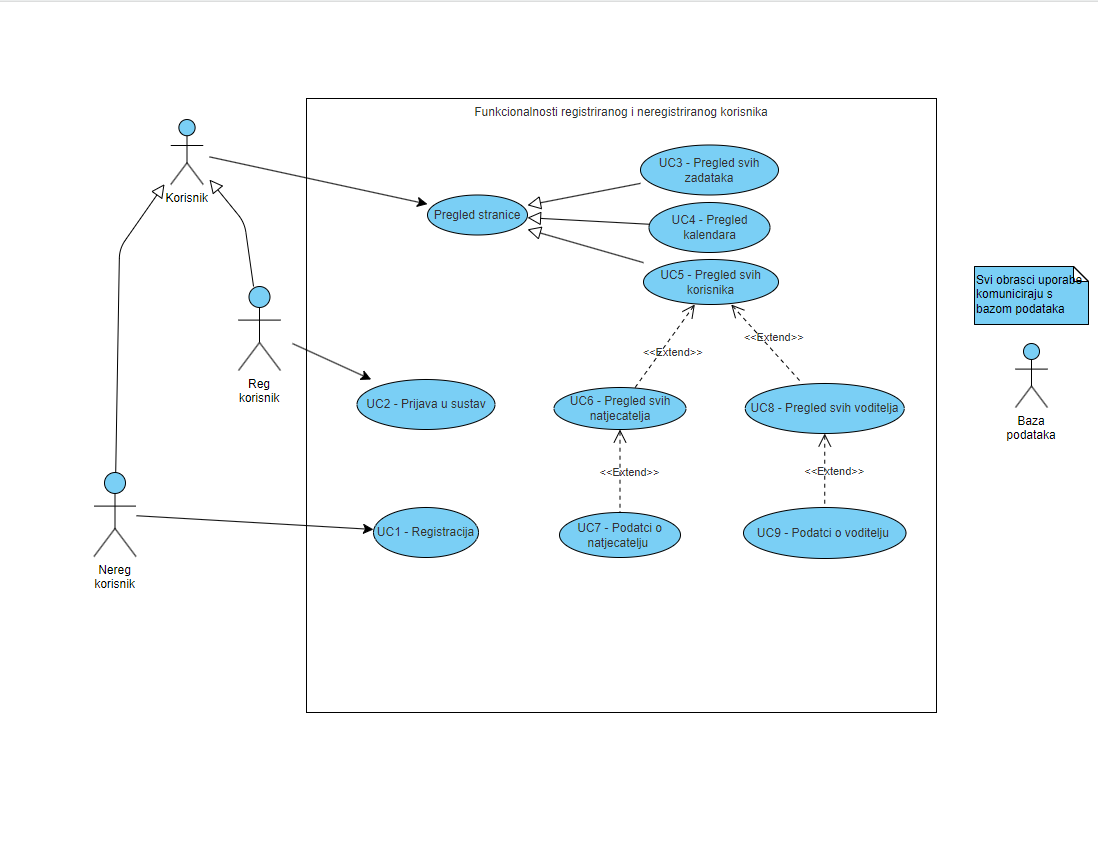
\includegraphics[scale=0.4]{slike/Uml - obrasci uporabe 1}
						%veličina slike u odnosu na originalnu datoteku i pozicija slike
						\centering
						\caption{Dijagram obrasca uporabe, funkcionalnost reg. i nereg. korisnika}
						\label{fig:dijagram1}
					\end{figure}
					
					\begin{figure}[H]
						\includegraphics[scale=0.4]{slike/Uml - obrasci uporabe 2}
						%veličina slike u odnosu na originalnu datoteku i pozicija slike
						\centering
						\caption{Dijagram obrasca uporabe, funkcionalnost voditelja, natjecatelja i administratora}
						\label{fig:dijagram2}
					\end{figure}
					
				\eject		
				
			\subsection{Sekvencijski dijagrami}
										
														
				\subsubsection{1) Registracija korisnika}
				
				\textbf{Opis dijagrama:}
				Korisnik započinje registraciju odabirom opcije "Registracija" na korisničkom sučelju. Nakon što korisnik odabere tu opciju, poslužitelj aplikacije šalje zahtjev korisniku da unese sljedeće podatke:
				
				\begin{itemize}
					\item (a) korisničko ime
					\item (b) fotografiju
					\item (c) lozinku
					\item (d) ime i prezime
					\item (e) email adresu
					\item (f) odabir: voditelj natjecanja / natjecatelj
				\end{itemize}
				
				Nakon što korisnik unese navedene podatke, šalje zahtjev za registraciju putem korisničkog sučelja. Nakon toga, poslužitelj provjerava unesene podatke. Provjerava  se dostupnost e-mail adrese i korisničkog imena u bazi podataka. U slučaju da su e-mail adresa ili korisničko ime već zauzeti, poslužitelj obavještava korisnika da registracija nije uspjela.
				U slučaju da su e-mail ili korisničko ime adresa dostupni, korisniku se šalje zahtjev za potvrdom registracije putem e-maila. Korisnik potvrđuje registraciju - podaci se trajno pohranjuju u bazu podataka, a poslužitelj obavještava korisnika da je registracija uspješna.
				
				U slučaju da se korisnik registrira kao "voditelj natjecanja," tada administrator mora u aplikaciji potvrditi novog voditelja. 
				
				\textbf{Slika dijagrama:}
				\begin{figure}[H]
					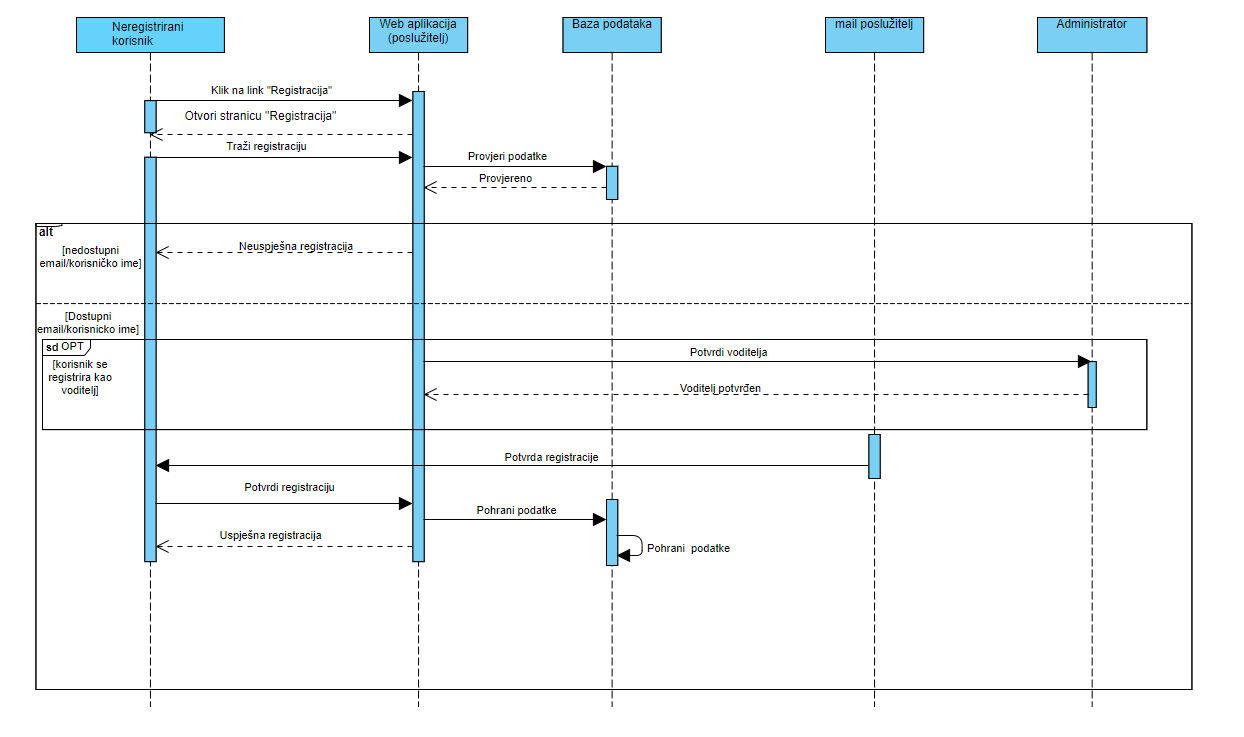
\includegraphics[scale=0.4]{slike/Registracija}
					%veličina slike u odnosu na originalnu datoteku i pozicija slike
					\centering
					\caption{Sekvencijski dijagram registracije novog korisnika}
					
				\end{figure}
				
				\subsubsection{2) Pregled i uređivanje korisnika}
				
				\textbf{Opis dijagrama:}
				Administrator šalje zahtjev za pregled korisnika i njihovih podataka tako da klikne na link "Pregled svih korisnika". Poslužitelj šalje upit bazi podataka za podatke registriranih korisnika, a baza podataka vraća podatke o registriranim korisnicima. Otvara se stranica s popisom registriranih korisnika i njihovim podacima koje je moguće urediti ili izbrisati. Kada administrator pošalje zahtjev za izmjenom podataka, podatci se uspješno pohranjuju u bazi podataka te se prikazuju na stranici. 
					
					\textbf{Slika dijagrama:}
					\begin{figure}[H]
					\centering
						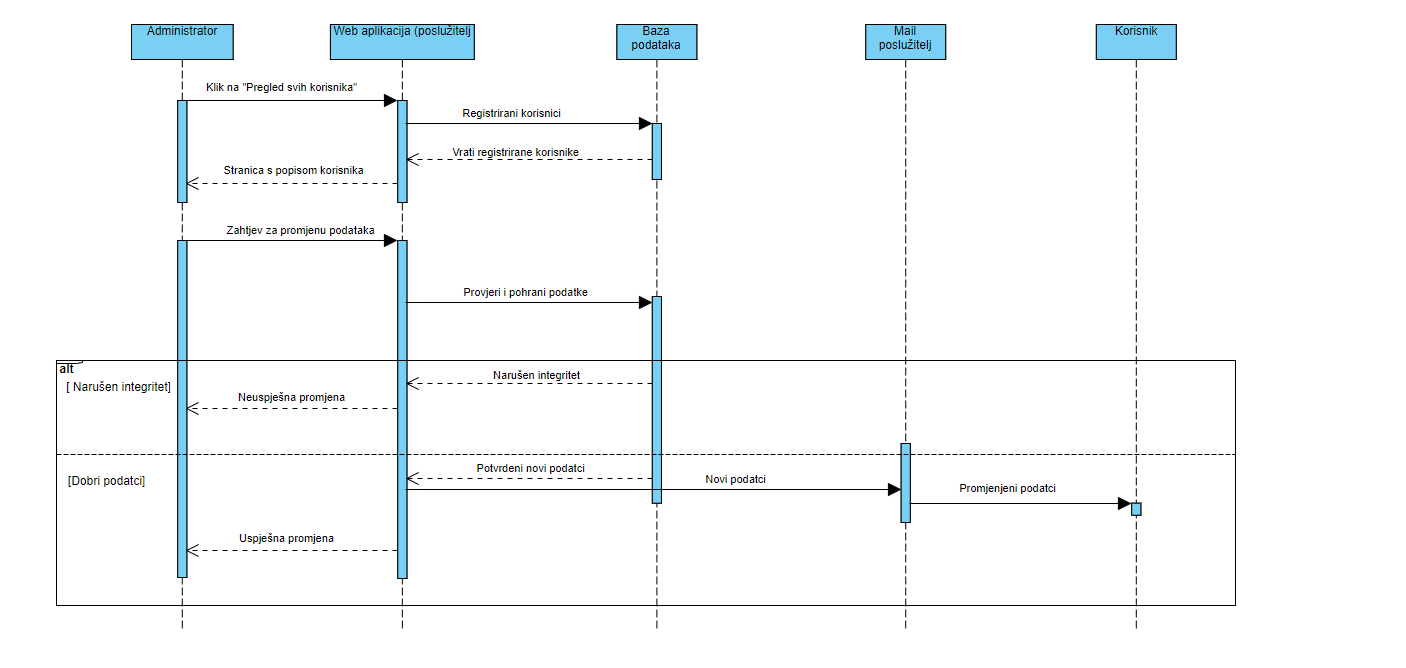
\includegraphics[scale=0.4]{slike/Pregled korisnika}
						%veličina slike u odnosu na originalnu datoteku i pozicija slike
						\centering
					\caption{Sekvencijski dijagram pregleda i uređivanja korisnika}
					\end{figure}
					
					\subsubsection{3) Virtualno natjecanje}
					
					\textbf{Opis dijagrama:}
					Kada natjecatelj klikne na link/gumb "Virtualno natjecanje", poslužitelj mu nudi mogućnost odabira između "Prethodno natjecanje" i "Nasumično odabrani zadaci".
					
					Ako natjecatelj odabere "Prethodno natjecanje", poslužitelj ga preusmjerava na kalendar natjecanja, gdje natjecatelj može birati prethodna natjecanja.
					
					Ako natjecatelj odabere opciju "Nasumično odabrani zadaci", poslužitelj iz baze podataka dohvaća zadatke i odabire ih ravnomjerno prema težini. Nakon odabiranja zadataka, zadaci se prikazuju natjecatelju.
					
					\textbf{Slika dijagrama:}
					\begin{figure}[H]
					\centering
					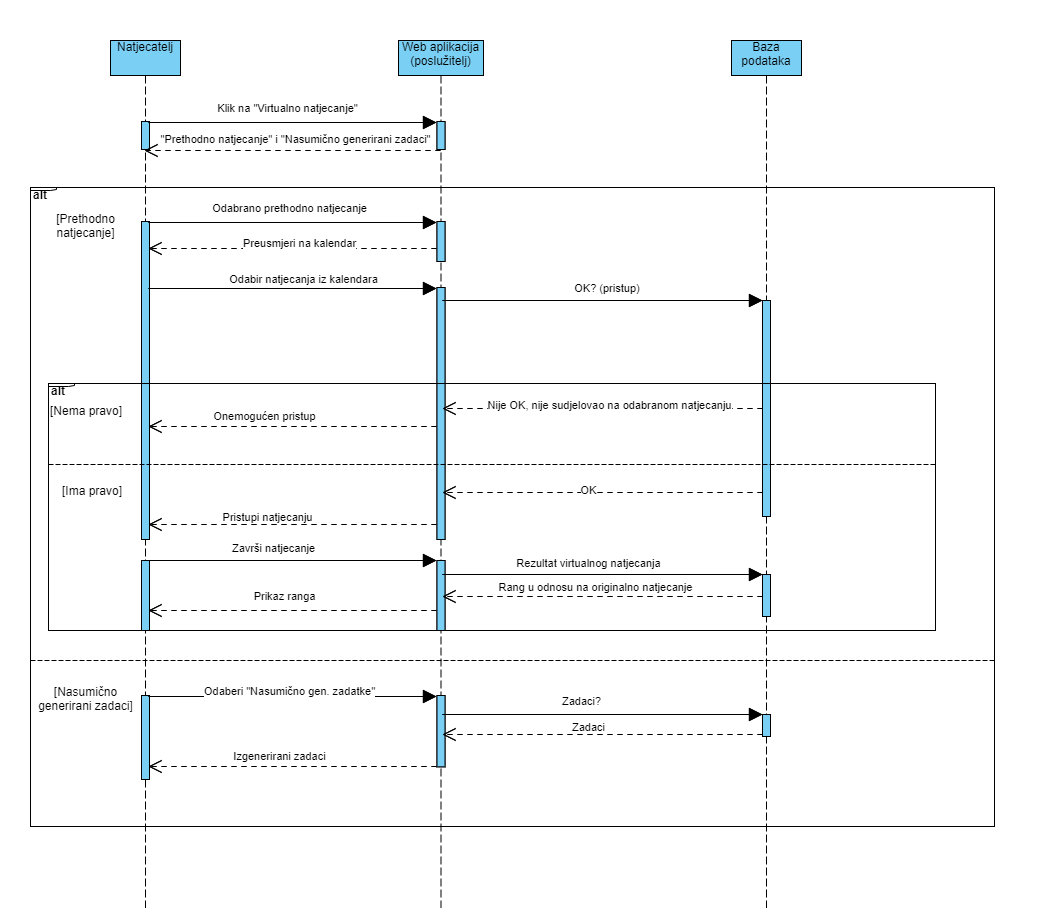
\includegraphics[scale=0.4]{slike/Virtualno natjecanje}
					%veličina slike u odnosu na originalnu datoteku i pozicija slike
					\caption{Sekvencijski dijagram virtualnog natjecanja}
					\end{figure}
			
					
				
				
	
		\section{Ostali zahtjevi}
		
			\begin{packed_item}
				\item Sustav treba biti funkcionalan na bilo kojem web pregledniku 
				\item Dohvat zadataka ili korisnika iz baze podataka mora se obaviti u konačnom vremenu (manji od 60 sekundi)
				\item Sustav mora podržavati hrvatsku abecedu pri unosu i prikazu tekstualnog sadržaja
				\item Sustav mora podržavati rad jednog ili više korisnika istovremeno  
				\item Pristup sustavu mora biti omogućen preko javne mreže pomoću HTTPS
				\item Nadogradnja sustava ne smije narušiti postojeće funkcionalnosti sustava 
				\item Sustav podržava format slike jpeg (maksimalna veličina 1048576 bajtova)
				\item Sustav mora podržavati programska rješenja u jeziku Java.
			\end{packed_item}
				
			
			 
			 
	